
\begin{figure}[ht]
    \centering
    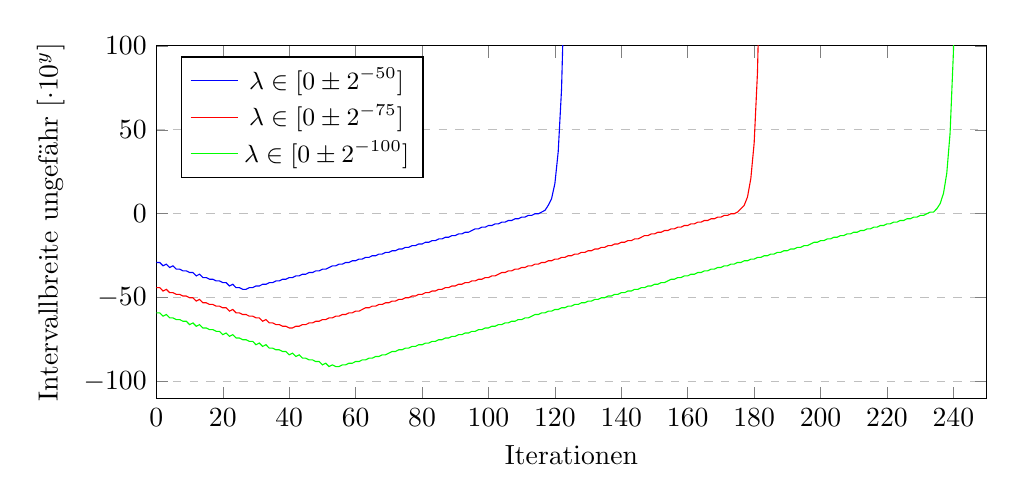
\begin{tikzpicture}
    \begin{axis}[
    width=\textwidth,
    height=0.5\textwidth,
        xlabel={Iterationen},
        ylabel={Intervallbreite ungefähr $[\cdot 10^y ]$},
        legend pos=north west,
        xmin=0,xmax=250,
        ymax=100,
        ymajorgrids=true,
        grid style=dashed,
    ]
    
    \addplot[
        color=blue,
        ]
        coordinates {
 (0,-29) (1,-29) (2,-31) (3,-30) (4,-32) (5,-31) (6,-33) (7,-33) (8,-34) (9,-34) (10,-35) (11,-35) (12,-37) (13,-36) (14,-38) (15,-38) (16,-39) (17,-39) (18,-40) (19,-40) (20,-41) (21,-41) (22,-43) (23,-42) (24,-44) (25,-44) (26,-45) (27,-45) (28,-44) (29,-44) (30,-43) (31,-43) (32,-42) (33,-42) (34,-41) (35,-41) (36,-40) (37,-40) (38,-39) (39,-39) (40,-38) (41,-38) (42,-37) (43,-37) (44,-36) (45,-36) (46,-35) (47,-35) (48,-34) (49,-34) (50,-33) (51,-33) (52,-32) (53,-31) (54,-31) (55,-30) (56,-30) (57,-29) (58,-29) (59,-28) (60,-28) (61,-27) (62,-27) (63,-26) (64,-26) (65,-25) (66,-25) (67,-24) (68,-24) (69,-23) (70,-23) (71,-22) (72,-22) (73,-21) (74,-21) (75,-20) (76,-20) (77,-19) (78,-19) (79,-18) (80,-18) (81,-17) (82,-17) (83,-16) (84,-16) (85,-15) (86,-15) (87,-14) (88,-14) (89,-13) (90,-13) (91,-12) (92,-12) (93,-11) (94,-11) (95,-10) (96,-9) (97,-9) (98,-8) (99,-8) (100,-7) (101,-7) (102,-6) (103,-6) (104,-5) (105,-5) (106,-4) (107,-4) (108,-3) (109,-3) (110,-2) (111,-2) (112,-1) (113,-1) (114,000) (115,000) (116,001) (117,002) (118,005) (119,009) (120,018) (121,037) (122,074) (123,147)
        };
        \addlegendentry{\small{$\lambda \in [0 \pm 2^{-50}]$}}
    
    \addplot[
        color=red,
        ]
        coordinates {
    (0,-44) (1,-44) (2,-46) (3,-45) (4,-47) (5,-47) (6,-48) (7,-48) (8,-49) (9,-49) (10,-50) (11,-50) (12,-52) (13,-51) (14,-53) (15,-53) (16,-54) (17,-54) (18,-55) (19,-55) (20,-56) (21,-56) (22,-58) (23,-57) (24,-59) (25,-59) (26,-60) (27,-60) (28,-61) (29,-61) (30,-62) (31,-62) (32,-64) (33,-63) (34,-65) (35,-65) (36,-66) (37,-66) (38,-67) (39,-67) (40,-68) (41,-68) (42,-67) (43,-67) (44,-66) (45,-66) (46,-65) (47,-65) (48,-64) (49,-64) (50,-63) (51,-63) (52,-62) (53,-62) (54,-61) (55,-61) (56,-60) (57,-60) (58,-59) (59,-59) (60,-58) (61,-58) (62,-57) (63,-56) (64,-56) (65,-55) (66,-55) (67,-54) (68,-54) (69,-53) (70,-53) (71,-52) (72,-52) (73,-51) (74,-51) (75,-50) (76,-50) (77,-49) (78,-49) (79,-48) (80,-48) (81,-47) (82,-47) (83,-46) (84,-46) (85,-45) (86,-45) (87,-44) (88,-44) (89,-43) (90,-43) (91,-42) (92,-42) (93,-41) (94,-41) (95,-40) (96,-40) (97,-39) (98,-39) (99,-38) (100,-38) (101,-37) (102,-37) (103,-36) (104,-35) (105,-35) (106,-34) (107,-34) (108,-33) (109,-33) (110,-32) (111,-32) (112,-31) (113,-31) (114,-30) (115,-30) (116,-29) (117,-29) (118,-28) (119,-28) (120,-27) (121,-27) (122,-26) (123,-26) (124,-25) (125,-25) (126,-24) (127,-24) (128,-23) (129,-23) (130,-22) (131,-22) (132,-21) (133,-21) (134,-20) (135,-20) (136,-19) (137,-19) (138,-18) (139,-18) (140,-17) (141,-17) (142,-16) (143,-16) (144,-15) (145,-15) (146,-14) (147,-13) (148,-13) (149,-12) (150,-12) (151,-11) (152,-11) (153,-10) (154,-10) (155,-9) (156,-9) (157,-8) (158,-8) (159,-7) (160,-7) (161,-6) (162,-6) (163,-5) (164,-5) (165,-4) (166,-4) (167,-3) (168,-3) (169,-2) (170,-2) (171,-1) (172,-1) (173,00) (174,00) (175,01) (176,03) (177,05) (178,10) (179,21) (180,42) (181,84) (182,168)
        };
        \addlegendentry{\small{$\lambda \in [0 \pm 2^{-75}]$}}
    
    \addplot[
        color=green,
        ]
        coordinates {
    (0,-59) (1,-59) (2,-61) (3,-60) (4,-62) (5,-62) (6,-63) (7,-63) (8,-64) (9,-64) (10,-66) (11,-65) (12,-67) (13,-66) (14,-68) (15,-68) (16,-69) (17,-69) (18,-70) (19,-70) (20,-72) (21,-71) (22,-73) (23,-72) (24,-74) (25,-74) (26,-75) (27,-75) (28,-76) (29,-76) (30,-78) (31,-77) (32,-79) (33,-78) (34,-80) (35,-80) (36,-81) (37,-81) (38,-82) (39,-82) (40,-84) (41,-83) (42,-85) (43,-84) (44,-86) (45,-86) (46,-87) (47,-87) (48,-88) (49,-88) (50,-90) (51,-89) (52,-91) (53,-90) (54,-91) (55,-91) (56,-90) (57,-90) (58,-89) (59,-89) (60,-88) (61,-88) (62,-87) (63,-87) (64,-86) (65,-86) (66,-85) (67,-85) (68,-84) (69,-84) (70,-83) (71,-82) (72,-82) (73,-81) (74,-81) (75,-80) (76,-80) (77,-79) (78,-79) (79,-78) (80,-78) (81,-77) (82,-77) (83,-76) (84,-76) (85,-75) (86,-75) (87,-74) (88,-74) (89,-73) (90,-73) (91,-72) (92,-72) (93,-71) (94,-71) (95,-70) (96,-70) (97,-69) (98,-69) (99,-68) (100,-68) (101,-67) (102,-67) (103,-66) (104,-66) (105,-65) (106,-65) (107,-64) (108,-64) (109,-63) (110,-63) (111,-62) (112,-62) (113,-61) (114,-60) (115,-60) (116,-59) (117,-59) (118,-58) (119,-58) (120,-57) (121,-57) (122,-56) (123,-56) (124,-55) (125,-55) (126,-54) (127,-54) (128,-53) (129,-53) (130,-52) (131,-52) (132,-51) (133,-51) (134,-50) (135,-50) (136,-49) (137,-49) (138,-48) (139,-48) (140,-47) (141,-47) (142,-46) (143,-46) (144,-45) (145,-45) (146,-44) (147,-44) (148,-43) (149,-43) (150,-42) (151,-42) (152,-41) (153,-41) (154,-40) (155,-39) (156,-39) (157,-38) (158,-38) (159,-37) (160,-37) (161,-36) (162,-36) (163,-35) (164,-35) (165,-34) (166,-34) (167,-33) (168,-33) (169,-32) (170,-32) (171,-31) (172,-31) (173,-30) (174,-30) (175,-29) (176,-29) (177,-28) (178,-28) (179,-27) (180,-27) (181,-26) (182,-26) (183,-25) (184,-25) (185,-24) (186,-24) (187,-23) (188,-23) (189,-22) (190,-22) (191,-21) (192,-21) (193,-20) (194,-20) (195,-19) (196,-19) (197,-18) (198,-17) (199,-17) (200,-16) (201,-16) (202,-15) (203,-15) (204,-14) (205,-14) (206,-13) (207,-13) (208,-12) (209,-12) (210,-11) (211,-11) (212,-10) (213,-10) (214,-9) (215,-9) (216,-8) (217,-8) (218,-7) (219,-7) (220,-6) (221,-6) (222,-5) (223,-5) (224,-4) (225,-4) (226,-3) (227,-3) (228,-2) (229,-2) (230,-1) (231,-1) (232,00) (233,01) (234,01) (235,03) (236,06) (237,12) (238,24) (239,48) (240,96) (241,192)
        };
        \addlegendentry{\small{$\lambda \in [0 \pm 2^{-100}]$}}
    
    
    
    
    
    
    \end{axis}
    \end{tikzpicture}
    \caption{Größenordnung der Breite des Kernintervalls bei der Berechnung von $x_{250}$ mit Sweeping square\_only}
    \label{fig:strategy2}
\end{figure}
